\section{Calibration: what chance means}\label{sec:calibration}

How many contacts would chance alone give? Pilots who never interact still meet: they take off
from the same site, follow the same ridges and climb in the same house thermals. A contact says
little by itself; what counts is how many contacts of a given duration occur beyond chance.
Interaction indices based on standard tests overestimate the interactions with finely
sampled telemetry~\cite{long2014}, so we build chance from the data, with copies of the flights shifted in
time, and derive from it the shortest duration $\tau^*$ of a contact. The run reported from here
on covers the 162\,485 cleaned flights of 6\,209 dates of the FFVL archive
(Section~\ref{sec:data}).

\subsection{The null model}\label{sec:null}

On each date we draw up to 200 pairs $(i,j)$ of flights whose takeoffs are less than $R_s=10$~km
apart, and replace flight $j$ by its copy shifted in time:
\begin{equation}\label{eq:shift}
  \x^s_j(t)=\x_j(t+r_{ij}),\quad z^s_j(t)=z_j(t+r_{ij}),\qquad
  r_{ij}=(k^0_j-k^0_i)-\vartheta,\quad \vartheta\sim\hat P\bigl(k^0_j-k^0_i\bigr).
\end{equation}
The delay $\vartheta$ is drawn from the delays between the takeoffs of the pairs of that date with
takeoffs within $R_s$: the copy of $j$ takes off $\vartheta$ after $i$, as a real pilot of the
day could. We accept only shifts with $|r_{ij}|\ge r_{\min}=2\delta+\Delta=245$~s, rounded to the
grid step, and a pair enters once, with the roles of $i$ and $j$ drawn at random. The idea of
shifting tracks in time, which keeps the spatial constraints and destroys the synchronisation,
comes from Spiegel et al.~\cite{spiegel2016}, who shuffle whole days of each individual; here a
flight is shifted within its day, against one other flight.

No real correspondence survives the shift (Figure~\ref{fig:null}). If $(t,t')$ was a real
correspondence, in the surrogate pair the position of $j$ at $t'$ comes at $t'-r_{ij}$, at least
$|r_{ij}|-\delta>\delta$ away from $t$. The correspondences that remain are encounters on the same
route without synchrony.

\begin{figure}
\centering
\begin{tikzpicture}[x=0.95cm,y=1cm]
  \foreach \y/\name in {2.2/real pair, 0.0/surrogate pair} \node[lbl, anchor=east] at (-0.2,\y+0.35) {\name};
  \begin{scope}[shift={(0,2.2)}]
    \draw[->, ink2] (0,0) -- (13.4,0) node[right, lbl, ink] {$t$};
    \fill[light] (5.0,-0.05) rectangle (7.0,0.95);
    \fill[blueI] (2.1,0.55) rectangle (10.1,0.75); \node[lbl, blueI, anchor=east] at (2.05,0.65) {$i$};
    \fill[orangeJ] (3.6,0.15) rectangle (12.1,0.35); \node[lbl, orangeJ, anchor=west] at (12.15,0.25) {$j$};
    \draw[ink, line width=0.8pt] (6.0,0.65) -- (6.7,0.25);
    \fill[ink] (6.0,0.65) circle (1.6pt) node[above, lbl] {$t$};
    \fill[ink] (6.7,0.25) circle (1.6pt) node[below right, lbl] {$t'$};
    \node[note] at (6.0,1.25) {$[t-\delta,t+\delta]$};
  \end{scope}
  \begin{scope}
    \draw[->, ink2] (0,0) -- (13.4,0) node[right, lbl, ink] {$t$};
    \fill[light] (5.0,-0.05) rectangle (7.0,0.95);
    \fill[blueI] (2.1,0.55) rectangle (10.1,0.75);
    \fill[orangeJ!55] (0.2,0.15) rectangle (8.7,0.35); \node[lbl, orangeJ, anchor=west] at (8.75,0.25) {$j$ shifted by $r_{ij}$};
    \fill[ink] (6.0,0.65) circle (1.6pt);
    \fill[ink] (3.3,0.25) circle (1.6pt) node[left=2pt, lbl, fill=white, inner sep=1pt] {$t'-r_{ij}$};
    \draw[->, ink2] (6.7,0.05) to[bend left=25] node[below, lbl] {$-r_{ij}$} (3.4,0.05);
  \end{scope}
\end{tikzpicture}
\caption{Null model. Top: a real correspondence $(t,t')$, with $t'$ inside the window
$[t-\delta,t+\delta]$ (grey). Bottom: $j$ shifted by $r_{ij}$, $|r_{ij}|>2\delta$; the same point
of $j$ now comes at $t'-r_{ij}$, outside the window.}
\label{fig:null}
\end{figure}

The shifted pair keeps the route, the terrain, the date, and the takeoff delays of the day as a
distribution. On the archive the shift is far larger than its minimum: 58~min in the median, and
90\% of the shifts lie between 8~min and 4.4~h (Figure~\ref{fig:shifts} in
Appendix~\ref{app:evidence}). So the copy also flies in the weather of another hour, with other
thermals working and another cloud base.

Chance is therefore an operational notion: the contacts that the same routes give without
synchrony. Two consequences follow.
\begin{itemize}
\item Pilots who use the same thermals at the same time without following each other share the
  weather of the hour, which the shift removes: their contacts count as real.
\item A pilot who follows another deliberately, but more than $\delta$ behind, never makes a
  contact in the real pair, while a surrogate whose shift brings that delay within $\delta$ counts
  it as chance.
\end{itemize}

\subsection{The false discovery rate and \texorpdfstring{$\tau^*$}{tau*}}\label{sec:fdr}

The surrogate pairs go through Phases~1--3 like the real ones (Appendix~\ref{sec:run}); their pair
intervals are the contacts chance alone gives. They are a sample of the pairs of each date, so we
count chance per second of exposure, date by date, and scale it to the real pairs. On date $d$:
\begin{itemize}
\item $\mathcal{P}_d$ is the set of the pairs $(a,b)$, $a<b$, of flights of the date with
  takeoffs less than $R_s$ apart; their exposure is $H_d=\sum_{\mathcal{P}_d}h_{ab}$, with
  $h_{ab}=\max\bigl(\min(k^\fin_a,k^\fin_b)-\max(k^\dep_a,k^\dep_b),\,0\bigr)$ the time both fly
  after departure;
\item $S_d$ is the same sum over the surrogate pairs $(i,j,r)$ of the date, with the times of $j$
  moved by $-r$;
\item $\rho_{0,d}(\tau)=M_d(\tau)/S_d$ is the number of chance intervals per second of exposure,
  with $M_d(\tau)$ the intervals of the surrogate pairs lasting at least $\tau$.
\end{itemize}
Over the archive, with $N(\tau)$ the number of real intervals of the pairs of every
$\mathcal{P}_d$ lasting at least $\tau$:
\begin{equation}\label{eq:fdr}
  C(\tau)=\sum_d \rho_{0,d}(\tau)\,H_d,\qquad
  \widehat{\mathrm{FDR}}(\tau)=\frac{C(\tau)}{N(\tau)},\qquad
  \tau^*=\min\bigl\{\tau:\ \widehat{\mathrm{FDR}}(\tau)\le q\bigr\}.
\end{equation}
Dates without surrogates add to $N$ only, and $\tau$ runs over the grid $\{0,5,\dots,14\,400\}$~s.

\begin{inwords}
$C(\tau)$ is the number of intervals lasting at least $\tau$ that chance alone would give the
real pairs. Dividing it by the number actually observed gives the share of chance intervals among
them; $\tau^*$ is the shortest duration at which that share falls to $q$, one in ten.
\end{inwords}

In analogy with SAM~\cite{tusher2001}, this is the number of discoveries expected by chance over
the number observed, with time shifts in place of the permutations.

\begin{figure}
\centering
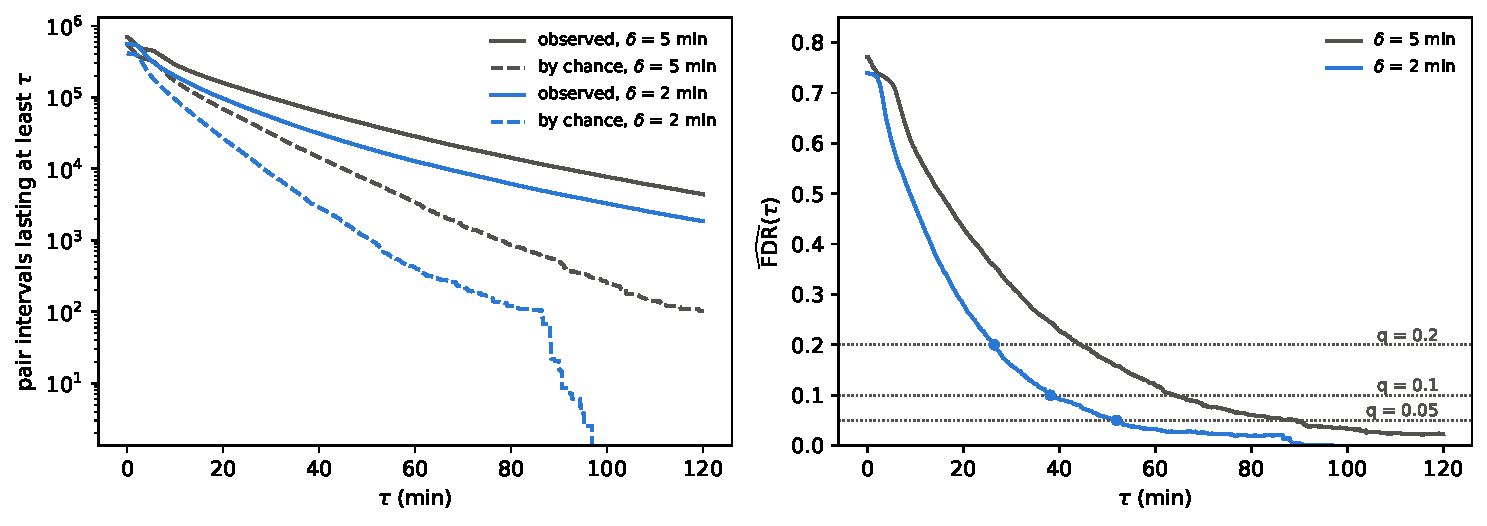
\includegraphics[width=\textwidth]{figures/assessment_fdr.pdf}
\caption{Left: real pair intervals lasting at least $\tau$ (solid) and those chance alone
gives (dashed), with $\delta=5$~min (grey) and $\delta=2$~min (blue), on the whole archive.
Right: their ratio, the false discovery rate of Eq.~\eqref{eq:fdr}; dots mark $\tau^*$ for
$q=0.05$, 0.1 and 0.2 with $\delta=2$~min.}
\label{fig:fdr}
\end{figure}

Most contacts are chance (Figure~\ref{fig:fdr}): 74\% of all pair intervals with
$\delta=2$~min (77\% with 5~min), 47\% of those lasting 10~min, 16\% of those lasting 30~min.
Short contacts say little; only long ones are mostly real. So $\tau^*$ is tens of minutes: it is
the duration at which the real contacts outnumber chance by the factor $1/q$. Resampling the dates
200 times moves $\tau^*$ by a few minutes (Table~\ref{tab:q}): the curve sets it, and the noise of
the surrogates barely moves it.

\subsection{How much the shift matters}\label{sec:shift-classes}

Does the length of the shift change what counts as chance? We recomputed the false discovery rate
with only the surrogate pairs of each date whose shift falls in one class, each class with its own
exposure $S_d$ and intervals, on the 2\,737 dates (of 6\,209) that have surrogates in every class
(Table~\ref{tab:shift-classes}).

\begin{table}
\centering
\small
\begin{tabular}{@{}l r c c c c@{}}
\toprule
Surrogates & pairs & $\widehat{\mathrm{FDR}}$(10 min) & $\widehat{\mathrm{FDR}}$(30 min) & $\tau^*$ (min) & 5--95\% over dates \\
\midrule
all shifts & 241\,824 & 0.48 & 0.16 & 38.2 & 37.0--41.5 \\
$|r|<30$ min & 69\,444 & 0.73 & 0.31 & 53.3 & 49.7--72.0 \\
$|r|\ge60$ min & 119\,687 & 0.26 & 0.05 & 23.0 & 21.1--24.4 \\
\bottomrule
\end{tabular}
\caption{The false discovery rate and $\tau^*$ ($q=0.1$, $\delta=2$~min) with the surrogates of
one class of shifts, on the 2\,737 dates with surrogates in each class.}
\label{tab:shift-classes}
\end{table}

It does, by more than a factor two. Short shifts give 2.8 times the chance of long ones at 10~min
and 5.7 times at 30~min, and $\tau^*$ goes from 23~min with shifts of an hour or more to 53~min
with shifts under 30~min; with all the shifts it is 38~min, as on the whole archive. Two effects
add up and cannot be separated here. Short shifts keep the weather of the hour, and they also
bring within $\delta$ the pilots who follow each other a few minutes apart, who are many: real
correspondences are still 2 to 3 times chance between 195 and 500~s
(Section~\ref{sec:delta-choice}).

\paragraph{What we keep.} Chance is what the same routes give without synchrony, with shifts that
follow the takeoff delays of the day. A contact counts only if it lasts at least $\tau^*$, the
duration at which at most a share $q$ of the contacts is chance; $q$ and $\delta$ are chosen in
Section~\ref{sec:tuning}.
